%--------------------------------------------------------------------
% NE 155 (intro to numerical simulation of radiation transport)

% formatting
\documentclass[12pt]{article}
\usepackage[top=1in, bottom=1in, left=1in, right=1in]{geometry}

\usepackage{setspace}
\onehalfspacing

\setlength{\parindent}{0mm} \setlength{\parskip}{1em}


% packages
\usepackage{amssymb}
%% The amsthm package provides extended theorem environments
\usepackage{amsthm}
\usepackage{epsfig}
\usepackage{times}
\renewcommand{\ttdefault}{cmtt}
\usepackage{amsmath}
\usepackage{graphicx} % for graphics files

% Draw figures yourself
\usepackage{tikz} 

% The float package HAS to load before hyperref
\usepackage{float} % for psuedocode formatting
\usepackage{xspace}

% from Denovo methods manual
\usepackage{mathrsfs}
\usepackage[mathcal]{euscript}
\usepackage{color}
\usepackage{array}

\usepackage{paralist, enumitem}

\usepackage[pdftex]{hyperref}

\newcommand{\nth}{n\ensuremath{^{\text{th}}} }
\newcommand{\ve}[1]{\ensuremath{\mathbf{#1}}}
\newcommand{\macro}{\ensuremath{\Sigma}}
\newcommand{\vOmega}{\ensuremath{\hat{\Omega}}}

\newcommand{\cc}[1]{\ensuremath{\overline{#1}}}
\newcommand{\ccm}[1]{\ensuremath{\overline{\mathbf{#1}}}}


%--------------------------------------------------------------------
%--------------------------------------------------------------------
\begin{document}
\begin{center}
{\bf NE 155, Classes 10, 11, \& 12 S17 \\
Differentiation \& Integration \\ February 8, 10, \& 13, 2017}
\end{center}

\setlength{\unitlength}{1in}
\begin{picture}(6,.1) 
\put(0,0) {\line(1,0){6.25}}         
\end{picture}

%--------------------------------------------------------------------
\section*{Differentiation}
We're building the skills required to solve
\begin{equation}
\frac{1}{v}\frac{\partial}{\partial t}\phi(\vec{r}, t) 
-\nabla \cdot D\nabla \phi(\vec{r}, t) + 
\Sigma_a \phi(\vec{r}, t) =
\nu \Sigma_f \phi(\vec{r}, t) +
S(\vec{r}, t) \:. \nonumber
\end{equation}
In practice, we can rarely get an analytical solution for $\phi$ so we have to solve it some other way. 
If we don't know what $\phi$ looks like, how do we take its derivative?
We need \textbf{numerical differentiation} so that we can come up with a way to express $\nabla^2 \phi$ or $\frac{\partial}{\partial t}\phi$ (or anything similar in any other equation).

\underline{Problem}: Given a function $f(x)$ at $x_0, x_1, \dots, x_n$, approximate $f'(x)$ or $f''(x)$, etc. 

Numerical differentiation is useful when a function is defined by 
\vspace*{-0.5em}
\begin{compactitem}
\item data
\item differential equations (ODEs, PDEs)
\end{compactitem}

\textbf{Example} Given $f$ is $ C^2 \in [a,b]$ and $x_0 \in [a,b]$, find an approximation to $f'(x_0)$.

We're going to come at this from \textbf{Taylor's theorem}, which gives an approximation of a k-times differentiable function around a given point by a k-th order Taylor polynomial.
% https://en.wikipedia.org/wiki/Taylor%27s_theorem

We'll start with a first order expansion for the point $x_0$:
\[
f(x) = f(x_0) + f'(x_0)(x - x_0) + \frac{f''(c)}{2}(x-x_0)^2 \]
\begin{align*}
% 
\therefore f'(x_0) &= \frac{f(x) - f(x_0)}{(x - x_0)} - \frac{f''(c)}{2}(x-x_0) \\
%
\text{Let } h &= x-x_0 \rightarrow x = x_0 + h \\
%
\therefore f'(x_0) &= \underbrace{\frac{f(x_0 + h) - f(x_0)}{h}}_{\text{computable approx.}} - \underbrace{\frac{f''(c)}{2}h}_{\text{error term}}
\end{align*}
%
We can extend this principle to get higher levels of accuracy. To do that we do a Taylor expansion for each point in our collection and choose how many points to combine and in what ways. 
%
\begin{center}
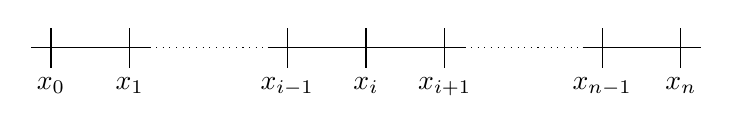
\begin{tikzpicture}
\draw (-.25,0)--(1.25,0);
\draw[dotted] (1.25,0)--(2.75,0);
\draw (2.75,0)--(5.25,0);
\draw[dotted] (5.25,0)--(6.75,0);
\draw (6.75,0)--(8.25,0);
%\draw (4,0)--(5.25,0);
\draw (0,-.25)--(0,.25);
\draw (1,-.25)--(1,.25);
%\draw (2,-.25)--(2,.25);
\draw (3,-.25)--(3,.25);
\draw (4,-.25)--(4,.25);
\draw (5,-.25)--(5,.25);
\draw (7,-.25)--(7,.25);
\draw (8,-.25)--(8,.25);
\node[below] at (0,-.25) {$x_0$};
\node[below] at (1,-.25) {$x_1$};
\node[below] at (3,-.25) {$x_{i-1}$};
\node[below] at (4,-.25) {$x_i$};
\node[below] at (5,-.25) {$x_{i+1}$};
\node[below] at (7,-.25) {$x_{n-1}$};
\node[below] at (8,-.25) {$x_n$};
\end{tikzpicture}
\end{center}
%
\vspace*{-2em}
\begin{align*}
f(x_i) &= f(x_i)\\
%
f(x_i \pm h) &= f(x_i) \pm hf'(x_i) + h^2\frac{f''(x_i)}{2} \pm h^3\frac{f'''(x_i)}{6} + f^{(4)}(c_1)\frac{h^4}{24} \\
%
f(x_i \pm 2h) &= f(x_i) \pm 2h f'(x_i) + 2 h^2 f''(x_i) \pm \frac{4}{3} h^3 f'''(x_i) + \frac{2}{3}h^4 f^{(4)}(c_2)
\end{align*}


% ---------------------------------------------------------
\subsection*{Forward difference:}
\underline{$O(h)$}: combine the point and the next point forward
\[f'(x_i) = \frac{f(x_i + h) - f(x_i)}{h} - \frac{1}{2}hf''(c)\]

\underline{$O(h^2)$}: combine the point and the next two points forward; we're going to need to figure out the coefficients though:

\begin{align*}
a f(x_i) &+ b f(x_i + h) + c f(x_i + 2h) = f'(x_i) \\
%
a f(x_i) &+ b[f(x_i) + hf'(x_i) + h^2\frac{f''(x_i)}{2} + h^3\frac{f'''(c_1)}{6}] \nonumber \\
&+ c[f(x_i) + 2h f'(x_i) + 2 h^2 f''(x_i) + \frac{4}{3} h^3 f'''(c_2)] =f'(x_i)\\
(a + b &+ c)f(x_i) + h(b + 2c)f'(x_i) + h^2(\frac{b}{2} + 2c) f''(x_i) \\
&+ h^3(\frac{b}{6} +  \frac{4c}{3}) f'''(\mu) = f'(x_i)
\end{align*}
%
Use mean value theorem to get $\mu \in [c_1, c_2]$ to be able to combine the error terms to get only one term.

*KEY* set the coefficients to get what we want:
%
\begin{align*}
(a + b + c) &= 0\\
h(b + 2c) &= 1\\
h^2(\frac{b}{2} + 2c) &= 0
\end{align*}
%
We don't have more degrees of freedom, so we're left with $f'''$ for the error term. 

Solving all of that gives
%
\begin{align*}
a &= -\frac{3}{2h} \\
b &= \frac{2}{h} \\
c &= -\frac{1}{2h} \\
&\text{error term } = -\frac{1}{3}h^2 f'''(\mu) \\
\therefore \quad &\boxed{f'(x_i) = \frac{-3 f(x_i) + 4f(x_i + h) - f(x_i + 2h)}{2h} -\frac{1}{3}h^2 f'''(\mu)}
\end{align*}


%--------------------------------------------------------------------
\subsection*{Backward difference:}
Essentially, the signs all flip because we use points in the other direction.

\underline{$O(h)$}: combine the point and the next point backward
\[f'(x_i) = \frac{f(x_i) - f(x_i - h)}{h} + \frac{1}{2}hf''(\mu)\]

\underline{$O(h^2)$}: combine the point and the next two points backward
%
\[f'(x_i) = \frac{3 f(x_i) - 4f(x_i - h) + f(x_i - 2h)}{2h} + \frac{1}{3}h^2 f'''(\mu)\]

%--------------------------------------------------------------------
\subsection*{Central difference:}
Use points on either side (the average of forward and backward difference) $\rightarrow$ more accuracy for the same number of evaluation  points.

\underline{$O(h^2)$}: combine one point on either side
\[f'(x_i) = \frac{f(x_i + h) - f(x_i - h)}{2h} - \frac{1}{6}h^2 f'''(\mu)\]

\underline{$O(h^4)$}: combine two points on either side
\[f'(x_i) = \frac{f(x_i - 2h) - 8f(x_i - h) + 8f(x_i + h) - f(x_i + 2h)}{2h} - \frac{1}{30}h^4 f^{(5)}(\mu)\]

\subsubsection*{Higher Order Derivatives}
By solving for different terms in the Taylor expansion, combining points, and solving for coefficients we can get other derivative terms as well. 

E.g. $a f(x_i + h) + b f(x_i) + c f(x_i - h) = f''(x_i)$

These are all $O(h^2)$:
\begin{align*}
f''(x_i) &= \frac{f(x_i - h) - 2f(x_i) + f(x_i + h)}{h^2} + \frac{h^2}{12}f^{(4)}(\mu) \\
%
f^{(3)}(x_i) &= \frac{-f(x_i - 2h) + 2f(x_i - h) - 2f(x_i + h) + f(x_i + 2h)}{2h^3}\\
%
f^{(4)}(x_i) &= \frac{f(x_i - 2h) - 4f(x_i - h) +6f(x_i) - 4f(x_i + h) + f(x_i + 2h)}{h^4}
\end{align*}

\subsubsection*{Two Variables}
\begin{align*}
\frac{\partial^2 f_{i,j}}{\partial x^2} = \frac{\partial}{\partial x}\bigl(\frac{\partial f_{i,j}}{\partial x}\bigr) =
\frac{f_{i-1,j} - 2f_{i,j} + f_{i+1,j}}{\Delta x^2} \\
%
\frac{\partial^2 f_{i,j}}{\partial y^2} = \frac{\partial}{\partial y}\bigl(\frac{\partial f_{i,j}}{\partial y}\bigr) =
\frac{f_{i,j-1} - 2f_{i,j} + f_{i,j+1}}{\Delta y^2}
\end{align*}
\begin{center}
\begin{tikzpicture}
\draw (-.25,0)--(7.25,0);
\draw (1,-.25)--(1,.25);
\draw (3,-.25)--(3,5.25);
\draw (4,-.25)--(4,5.25);
\draw (5,-.25)--(5,5.25);
\draw (7,-.25)--(7,.25);
\node[below] at (0,-.25) {$x_i$};
\node[below] at (1,-.25) {$x_1$};
\node[below] at (3,-.25) {$x_{i-1}$};
\node[below] at (4,-.25) {$x_i$};
\node[below] at (5,-.25) {$x_{i+1}$};
\node[below] at (7,-.25) {$x_n$};
\node at (3.5, 2) {$\Delta x$};
% begin y
\draw (0,-.25)--(0,7.25);
\draw (-.25,1)--(.25,1);
\draw (-.25,3)--(5.25,3);
\draw (-.25,4)--(5.25,4);
\draw (-.25,5)--(5.25,5);
\draw (-.25,7)--(.25,7);
\node[left] at (-.25, 0) {$y_0$};
\node[left] at (-.25,1) {$y_1$};
\node[left] at (-.25,3) {$y_{j-1}$};
\node[left] at (-.25,4) {$y_j$};
\node[left] at (-.25,5) {$y_{j+1}$};
\node[left] at (-.25,7) {$y_n$};
\node at (2,3.5) {$\Delta y$};
\end{tikzpicture}
\end{center}


%--------------------------------------------------------------------
%-------------------------------------------------------------------
\vspace*{-2em}
\section*{Integration}
Why might we need to numerically integrate?
\begin{itemize}
\item The integrand, $f(x)$, is complicated enough that its
indefinite or even definite integral over a particular range cannot
be found.
\item The indefinite or definite integral can be found, but may take
long time to calculate analytically.
\item The integrand is given in terms of a table. That is, we are
provided with discrete values of $f(x)$ at $n+1$ data points.
\end{itemize}

For us, we use this particularly for the scattering and fission in the Transport Equation:
\[\int_{4\pi} d\vOmega' \int_0^{\infty} dE' \Sigma_s(E', \vOmega' \rightarrow E, \vOmega) \psi(\vec{r}, E', \vOmega', t)  +
 \frac{\chi(E)}{4\pi} \int_0^{\infty} dE' \nu(E') \Sigma_f(E') \int_{4\pi} d\vOmega' \psi(\vec{r}, E', \vOmega', t) \]

The general strategy is:
\begin{itemize}
\item Approximate the integrand $f(x)$ with either a global interpolating
polynomial defined over the whole domain of integration, or a
collection of local interpolating polynomials defined over intervals
that are subtended by a small group of data points.
\item Integrate the interpolating polynomial(s) over their individual
domains of definition.
\end{itemize}

Thus, given $f \in[a,b]$, compute $I(f) = \int_a^b f(x) dx$.

The way we do this is called \textbf{numerical integration} or \textbf{numerical quadrature}:
\[I(f) \approx I_n(f) = \sum_{i=0}^n w_i f(x_i)\]
\vspace*{-3em}

$w_i \equiv$ quadrature weights\\
$x_i \equiv$ quadrature points

\textbf{Approach \#1}\\
Fix quadrature points ($x_i$), then choose quadrature weights ($w_i$). Usually fit a polynomial to $f(x_i)$ and integrate.
%
\begin{enumerate}%[a.]
\item \underline{Newton-Cotes}: use a single poly over the entire interval
\item \underline{composite Newton-Cotes}: split the interval
\item \underline{Romberg integration}: extrapolation
\end{enumerate}

\textbf{Approach \#2}\\
For a given $n$, choose the ``best" quadrature points ($x_i$) and quadrature weights ($w_i$):\\
\underline{Gaussian Quadrature}

\vspace*{1em}
the \textbf{degree of precision} of a quadrature formula, $I_n(f)$, is the positive integer $m$ s.t.:
\begin{enumerate}
\item $I(p) = I_n(p)$ for every poly of degree $\leq m$.
\item $I(p) \neq I_n(p)$ for some poly of degree $m+1$.
\end{enumerate}
 
 
%--------------------------------------------------------------------
\subsection*{Newton-Cotes formula}
 
\underline{idea}: fix $x_0, x_1, \dots, x_n$ then interpolate $f(x)$ by a poly of degree $\leq n$.
%
\begin{align*}
I(f) &\approx I_n(f) = I(p_n)\\
\text{true integral } &\approx \text{ N-C formula } = \text{ true integral of interpolating poly}
\end{align*}
%
The only error is in the polynomial interpolation.

%--------------------------------------------------------------------
\subsection*{Lagrange form of NC}
Choosing Lagrange polynomials prevents us from needing to recalculate weights for every $f(x)$ (since we've fixed the points). Note, we're assuming equally spaced points: $h = (b-a)/n$. This is not a necessary assumption, but indexing of $h$ would be required for unequally spaced points.
%
\begin{align*}
P_n(x) &= \sum_{i=0}^{n}f(x_i)L_i(x) \\
%
I(P_n(x)) &= \sum_{i=0}^{n} \bigl[ \int_a^b L_i(x)dx \bigr] f(x_i) \\
%
&= \sum_{i=0}^{n} w_i f(x_i)\\
\text{where } w_i &=  \int_a^b L_i(x)dx = \int_a^b \prod_{\substack{i=0\\ i \neq k}}^n \frac{(x-x_i)}{(x_k-x_i)} \\
&\text{sub in } x = a + sh\\
&=  (b-a)\frac{1}{n}\int_0^n \prod_{\substack{i=0\\ i \neq k}}^n \frac{(s-i)}{(k-i)}ds
\end{align*}
We can see $w_i$ are not dependent on $f(x)$.

%--------------------------------------------------------------------
\subsubsection*{Trapezoid Rule}
This is the Lagrange form of Newton-Cotes integration with $n=1$.

$x_0 = a$, $x_1 = b$, $h = x_1 - x_0$
%
\begin{align*}
&L_0(x) = \frac{x-x_1}{x_0-x_1}\:, \qquad L_1(x) = \frac{x-x_0}{x_1-x_0} \\
%
w_0 &= \int_{x_0}^{x_1} \bigl(\frac{x-x_1}{x_0-x_1}\bigr) dx\:; 
\\ &\text{let } x = x_0 + th  \:, \quad dx = h\:dt\:, \quad t = \frac{x-x_0}{h}\:,\\
&\text{change bounds and note that the denominator is }-h \\
%
w_0 &= h \int_0^1 \bigl(\frac{x_1 - x_0 - ht}{h}\bigr)dt = \int_0^1 h(1-t)dt \\
%
w_0 &= h\bigl(t - \frac{1}{2}t^2 \bigr) |_0^1 = \frac{1}{2}h\\
%
w_1 &= \int_{x_0}^{x_1} \bigl(\frac{x-x_0}{x_1-x_0}\bigr) dx = \frac{1}{2}h\\
%
\therefore I_1(f) = w_0f(x_0) &+ w_1f(x_1)  = \boxed{\frac{h}{2}\bigl(f(x_0) + f(x_1)\bigr)} \rightarrow \text{area of a trapezoid}
\end{align*}
%
The trapezoid rule has degree of precision 1.

\begin{figure}
\begin{center}
  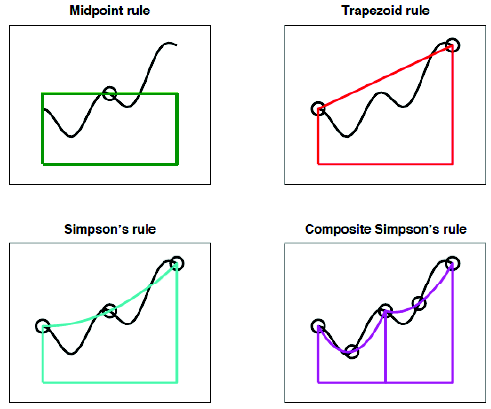
\includegraphics[height=4in,clip]{QuadratureComparison}
\end{center}
\caption{examples of how different integration rules capture a function}
\end{figure}

%--------------------------------------------------------------------
\subsubsection*{Error Analysis}
\begin{enumerate}
\item interpolate:
\[f(x) = P_n(x) + R_n(x)\]
\item integrate:
\[\underbrace{\int_a^b f(x) dx}_{I(f)} = \underbrace{\int_a^b P_n(x)dx}_{I_n(f)} + \int_a^b R_n(x) dx\]
\end{enumerate}

\textbf{Example:} Trapezoid Rule\\
Recall from Lagrange polynomials that we know how to express $R_n$. We can then use that to compute the error of the integral.
\begin{align*}
R_1(x) &= \frac{f''(c)}{2!}(x-x_0)(x-x_1) \\
I(f) - I_1(f) &= \int_{x_0}^{x_1} \frac{f''(c)}{2!}\underbrace{(x-x_0)(x-x_1)}_{\text{doesn't change sign over interval}} dx
\end{align*}
%
Recall that $c$ depends on $x$. To get an expression, we're going to use the mean value theorem (which I briefly referenced last time).

\underline{Mean Value Theorem for Integrals}\\
\[\int_a^b f(x)g(x)dx = f(\xi) \int_a^b g(x)dx\:, \qquad a\leq \xi \leq b\]
Where $g(x)$ must always be positive or always negative (cannot change sign over the interval).

Thus, we can use MVT for our integral to see that
\begin{align*}
I(f) - I_1(f) &= \frac{1}{2}f''(\eta) \int_{x_0}^{x_1} (x-x_0)(x-x_1) dx \\
&= \frac{1}{2}f''(\eta) \bigl(\frac{-h^3}{6}\bigr) \rightarrow \boxed{\frac{-h^3}{12}f''(\eta)}
\end{align*}
is the error term for trapezoid rule. You can see that this has \underline{degree of precision 1 b/c the second derivative} \underline{drives the error} and \textit{the error changes as $O(h^3)$ with mesh spacing}.


%--------------------------------------------------------------------
\vspace*{-1em}
\subsubsection*{Simpson's Rule}
This is the Lagrange form of Newton-Cotes integration with $n=2$.

\begin{align*}
x_0 &= a \qquad x_1 = \frac{a+b}{2} \qquad x_2=b \qquad h=\frac{b-a}{2}\\
%
L_0 &= \frac{(x-x_1)(x-x_2)}{(x_0-x_1)(x_0-x_2)}\\
L_1 &= \frac{(x-x_0)(x-x_2)}{(x_1-x_0)(x_1-x_2)}\\
L_2 &= \frac{(x-x_0)(x-x_1)}{(x_2-x_0)(x_2-x_1)}\\
%
w_0 &= \int_{x_0}^{x_2} L_0(x)dx = \frac{h}{3}\\
w_1 &= \int_{x_0}^{x_2} L_1(x)dx = \frac{4h}{3}\\
w_2 &= \int_{x_0}^{x_2} L_2(x)dx = \frac{h}{3}\\
&\text{Note: weights sum to }2h\text{, the size of the interval}\nonumber\\
%
&\therefore I_2(f) = \frac{h}{3}\bigl(f(x_0) + 4f(x_1) + f(x_2)\bigr) 
\end{align*}
 
The error term comes from integrating $R_2 = \frac{1}{3!}f'''(c)(x-x_0)(x-x_1)(x-x_2)$. However, the middle term now changes sign over the interval and we can't just use MVT.

We're going to skip the details, but what we get out is that the error for Simpson's Rule looks like:
\[\frac{-f^{(4)}(\eta)}{4!}\frac{h^5}{\frac{4}{15}} \rightarrow \boxed{\frac{-f^{(4)}(\eta)}{90}h^5}\]

Thus, Simpson's rule has degree of precision 3 and is $O(h^5)$.

\textbf{In General:}
\vspace*{-1em}
\begin{center}
\begin{tabular}{c c c}
$n$  & error        & precision \\ \hline
odd  & $O(h^{n+2})$ & $n$ \\
even & $O(h^{n+3})$ & $n+1$ \\
\end{tabular}
\end{center}

\underline{Simpson's 3/8 rule}:\\
If $n=3$:
\[\int_{x_0}^{x_3} f(x)dx = \frac{3h}{8}\bigl(f(x_0) + 3f(x_1) + 3f(x_2) + f(x_3)\bigr) - \frac{3h^5}{80}f^{(4)}(\xi)\]
where $x_0 < \xi < x_3$ and $h=(x_3 - x_0)/3$.

%--------------------------------------------------------------------
\subsubsection*{Composite Newton-Cotes}
Some difficulties:
\begin{enumerate}
\item To add points we must recompute the weights, $w_i$, which can be a lot of work.
\item high order polynomial interpolation on equally spaced points is BAD. (using optimally-spaced points is Gaussian quadrature; we'll get to that later).
\end{enumerate}

\underline{Idea:} subdivide $[a,b]$ into subintervals. On each of these apply a low-order Newton-Cotes formula.

\textbf{Composite Trapezoid}:\\
Just apply the trapezoid rule on each subinterval. Given $x_0, x_1, \dots, x_n$ and $f(x_0), f(x_1), \dots f(x_n)$, the grid space is $h = \frac{x_n-x_0}{n}$.

\textit{DRAW PICTURE}
\vspace*{-1em}
\begin{align*}
\int_{a}^{b} f(x)dx &= \sum_{i=1}^n \int_{x_{i-1}}^{x_i} f(x)dx\\
&= \sum_{i=1}^n \bigl[ \frac{h}{2}\bigl(f(x_{i-1}) + f(x_i)\bigr) - \frac{h^3}{12}f''(c_i) \bigr] \\
&= \frac{h}{2}\bigl(f(a) + 2\sum_{i=1}^{n-1}f(x_i) + f(b)\bigr) - \frac{h^3}{12} \underbrace{\sum_{i=1}^n f''(c_i)}_{\substack{n f''(\mu),\\ n = (b-a)/h}}\\
\int_{a}^{b} f(x)dx &= \boxed{\frac{h}{2}\bigl(f(a) + 2\sum_{i=1}^{n-1}f(x_i) + f(b)\bigr) - \frac{h^2}{12}(b-a)f''(\mu) }
\end{align*}
 
\textbf{Composite Simpson}:\\
Similarly, apply the Simpson rule on each subinterval. Note that for the functionally-equivalent sense of $n$ intervals we really need to use $2n$ points since each Simpson is applied using 3 points, and the end points are re-used. Therefore $\int_{a}^{b} f(x)dx = $
%
\begin{align*}
\sum_{i=1}^{n/2}\int_{x_{2i-1}}^{x_{2i}} f(x)dx &= \sum_{i=1}^{n/2} \bigl[ \frac{h}{3}\bigl(f(x_{2i-2}) + 4f(x_{2i-1}) + f(x_{2i})\bigr) - \frac{f^{(4)}(c_i)}{90}h^5 \bigr]\\
&\quad \text{MVT: } \sum_{i=1}^{n/2}f^{(4)}(c_i) = \frac{n}{2}f^{(4)}(\mu) = \frac{b-a}{2h}f^{(4)}(\mu)\\
&= \frac{h}{3}\bigl(f(a) + \underbrace{4\sum_{i=1}^{n/2} f(x_{2i-1})}_{\text{odd points}} + \underbrace{2\sum_{i=1}^{n/2-1} f(x_{2i})}_{\text{even points}} + f(b)\bigr) - \frac{h^4}{180}(b-a)f^{(4)}(\mu)
\end{align*}


%--------------------------------------------------------------------
\subsubsection*{Open Newton-Cotes}
The previous examples were called \textbf{closed} Newton-Cotes because $f(x)$ is evaluated at the first and last points.

\textbf{Open} Newton-Cotes does not evaluate $f(x)$ at the endpoints. The node points are still defined as $x_{j} = x_0 + jh, j = 0, \dots, n$,  but now 
\vspace*{-1em}
\begin{center}
\begin{tabular}{c c c}
Item & Open & Closed \\ \hline
$h$  & $\frac{b-a}{n+2}$ & $\frac{b-a}{n}$ \\
$x_0$ & $a+h$ & $a$ \\
$x_n$ & $b-h$ & $b$ \\
\end{tabular}
\end{center}
%
Now our real endpoints are $x_{-1}$ and $x_{n+1}$ (so we're doing $\int_{x_{-1}}^{x_{n+1}} f(x)dx$), which gives
\[
 w_i =  \int_a^b L_i(x)dx = \int_a^b \prod_{\substack{i=0\\ i \neq k}}^n \frac{(x-x_i)}{(x_k-x_i)} =  (b-a)\frac{1}{n+2}\int_0^n \prod_{\substack{i=0\\ i \neq k}}^n \frac{(s-i)}{(k-i)}ds
 \]

\begin{figure}
\begin{center}
  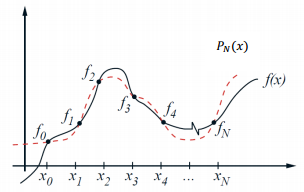
\includegraphics[height=2in,clip]{ClosedNewtonCotes}
  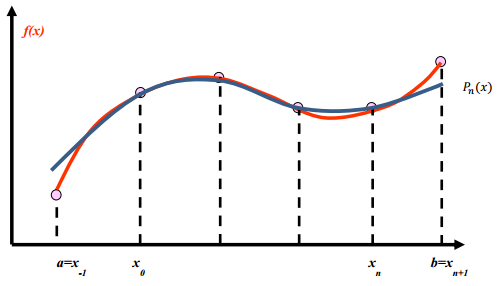
\includegraphics[height=1.75in,clip]{OpenNewtonCotes}
\end{center}
\caption{[left] example of \textbf{closed} Newton Cotes (where the interpolation \textit{matches} at the end points); [right] example of \textbf{open} Newton Cotes (where the interpolation \textit{does not match} at the end points)}
\end{figure}

%A quick explanation of difference I've found on slides 17 and 18:\\ \href{http://www.math.uconn.edu/~leykekhman/courses/MATH_5520/Notes/quadrature_1.pdf}{http://www.math.uconn.edu/$\sim$leykekhman/courses/MATH\_5520/Notes/quadrature\_1.pdf}

\vspace*{1 em}
The \underline{midpoint rule} is what we get with \underline{$n=0$}; it only uses one point:
\[\int_a^b f(x)dx = \int_{x_{-1}}^{x_{1}} f(x)dx = 2hf(x_0) + \frac{h^3}{3}f''(\xi)\]
where $x_{-1} < \xi < x_{1}$ and $h=(b-a)/2$.

\underline{$n=1$}:
\[ \int_{x_{-1}}^{x_{2}} f(x)dx = \frac{3h}{2}[f(x_0) + f(x_1)] + \frac{3h^3}{4}f''(\xi)\]
where $x_{-1} < \xi < x_{2}$ and $h=(b-a)/3$.

\underline{$n=2$}:
\[ \int_{x_{-1}}^{x_{3}} f(x)dx = \frac{4h}{3}[2f(x_0) - f(x_1) + 2f(x_2)] + \frac{14h^5}{45}f^{(4)}(\xi)\]
where $x_{-1} < \xi < x_{3}$ and $h=(b-a)/4$.




%--------------------------------------------------------------------
%--------------------------------------------------------------------
%\bibliographystyle{plain}
%\bibliography{LinearSolns} 

\end{document}